\documentclass{beamer}
%[aspectratio=169]   \usepackage[czech]{babel}
\usepackage{apo-lecture}
\usepackage{pdfpages}
\usepackage{pdfcomment}
\usepackage{listings}
\usepackage{array,multirow}

\subtitle{Lekce 04. Hierarchie paměti}
\author{Pavel Píša \phantom{xxxxxxx} Petr Štěpán \\ \small\texttt{pisa@fel.cvut.cz}\phantom{xxxx}\small\texttt{stepan@fel.cvut.cz}}
\begin{document}

\maketitle

\section{Druhy paměti}

\begin{frame}[fragile]
\frametitle{Motivace}

\begin{columns}
\begin{column}{0.45\textwidth}
Algoritmus A\\
\begin{minted}{c}
int matrix[N][N];
int main() {
  long int i, j, sum1 = 0;
  for(i=0; i<N; i++)
    for(j=0; j<N; j++)
      sum1 += matrix[i][j];
}
\end{minted}
\end{column}
\hfill
\begin{column}{0.45\textwidth}
Algoritmus B\\
\begin{minted}{c}
int matrix[N][N];
int main() {
  long int i, j, sum1 = 0;
  for(i=0; i<N; i++)
    for(j=0; j<N; j++)
      sum1 += matrix[j][i];
}
\end{minted}
\end{column}
\end{columns}
\bigskip
Oba dva programy vypadají velmi podobně. 

Program A prochází pole po řádcích, program B prochází pole po sloupcích.
\bigskip

Bude se nějak lišit doba výpočtu?

\end{frame}

\begin{frame}[fragile]
\frametitle{Motivace}

\begin{columns}
\begin{column}{0.45\textwidth}
Algoritmus A\\
\begin{minted}{c}
int matrix[N][N];
int main() {
  long int i, j, sum1 = 0;
  for(i=0; i<N; i++)
    for(j=0; j<N; j++)
      sum1 += matrix[i][j];
}
\end{minted}
\end{column}
\hfill
\begin{column}{0.45\textwidth}
Algoritmus B\\
\begin{minted}{c}
int matrix[N][N];
int main() {
  long int i, j, sum1 = 0;
  for(i=0; i<N; i++)
    for(j=0; j<N; j++)
      sum1 += matrix[j][i];
}
\end{minted}
\end{column}
\end{columns}
\bigskip

\begin{tabular}{|l|l|l|}\hline
N & A & B \\\hline
100000 & 12.791328s &138.047563s \\\hline
10000 & 0.126945s &0.486535s \\\hline
1000 & 0.001329s &0.001756s \\\hline
100 & 0.000083s &0.000094s \\\hline
\end{tabular}
\end{frame}


\begin{frame}
\frametitle{Co je paměť}

Paměť :
\begin{itemize}
\item je pole adresovatelných buněk
\begin{itemize}
\item každá buňka obsahuje jeden bajt - tedy 8 bitů
\end{itemize}
\item velikost paměti je omezena jak velkou adresu je CPU schopno nastavit na paměťové sběrnici, tedy kolik bitů lze použít k adresování paměti
\begin{itemize}
\item 16 bitů adresy umožňuje maximálně 64KiB velkou paměť
\item 32 bitů adresy umožňuje maximálně 4GiB velkou paměť
\item 37 bitů adresy (maximum procesoru Intel Core i9, pak záleží ještě na základní desce) maximálně 128 GiB velkou paměť
\end{itemize}
\item typ přístupu:
\begin{itemize}
\item k vnitřní paměti počítače lze přistupvat v náhodném pořadí (= random access)
\item některé externí paměti (např. magnetopásková paměť využívaná pro zálohování -- levnější než HDD a SSD) umožňjí pouze sekvenční přístup, tedy čtení a zápis bajtů po sobě
\end{itemize}
\end{itemize}

\end{frame}


\begin{frame}
\frametitle{Druhy paměti}

Paměti dělíme podle možností zápisu na:
\begin{itemize}
\item \textbf{ROM} (Read-Only Memory) paměti ze kterých lze pouze číst, řadíme sem i paměti typu EEPROM (Electrically Erasable Programmable Read-Only Memory), které lze omezeně smazat vysokým napětím a pak tam zapsat nové údaje, při normálním provozu nejde do paměti zapsat.
\item \textbf{RAM} (Random Access Memory) také RWM (Read-Write Memory) lasické paměti určené pro čtení a zápis libovolné buňky v libovolném pořadí -- Random Access.
\end{itemize}

Paměti lze dělit i podle toho, zda data jsou uchována po vypnutí napájení:
\begin{itemize}
\item \textbf{Permanentní} (Non-volatile) paměť nepotřebuje k udržení informace napájení - např. 3D-X Point -- Intel Optane Memory, feromagnetické paměti, HDD, SSD, 
\item \textbf{Volatilní} (Volatile) například paměť DDR v klasickém počítači, k udržení informace je potřeba nepřetržité napájení a obnova dat.
\end{itemize}
\end{frame}

\begin{frame}
\frametitle{Konstrukce paměti}

Podle kontrukce dělíme paměti RAM (RWM) na:
\bigskip

\begin{tabular}{b{0.8cm}m{6cm}m{4cm}}
SRAM & Statická RAM -- veličina reprezentující hodnotu má v čase konstatní hodnotu. Typicky dva do smyčky zapojené invertory. Více součástek dražší paměť, nemusí se obnovovat uložená informace, potřebuje pouze napájení & 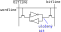
\includegraphics[width=3.8cm]{sram.pdf} \\ 
\phantom{x} & & \\
DRAM & Dynamická RAM -- veličina mění v čase svoji hodnotu. Typicky kondezátor, který se samovolně vybíjí a je proto nutné informaci obnovovat v pravidelných časech. Pouze kondenzátor a tranzistor -- levné, zabere méně prostoru. & \includegraphics[width=3.2cm]{dram.pdf}\\
\end{tabular}

\end{frame}

\end{document}

